\chapter{Results}
\label{ch:results}

In this chapter, we showcase the pipeline we have managed to create on a simple, low polygon-count model. We also attach all the necessary files to recreate the steps taken here. We use a model downloaded from the internet, which is the expected use case of our application.

\section{Acquiring and preprocessing the model}

As a beginner, the user will not create his own model, but download the free ones from the internet. Here we hope to demonstrate the pipeline from the user's perspective, so we will do the same. We will be using this model \footnote{https://www.thingiverse.com/thing:327753} from Thingiverse \footnote{https://www.thingiverse.com}.

Before we can get to Pepr3D, we unfortunately have to pre-process the model somewhat, as the artist forgot to specify the model's normals. This is a very easy correction in Blender, but already showcases the fact, that the models found on the internet suffer from a plethora of problems, some of which are detectable and correctable within the program and some of which are not. We attach the already corrected .STL file as well.

\section{Loading the model into Pepr3D}

Once we have our model cleaned up -- removing all duplicate vertices, reducing the model to a manifold object and making sure the normals are pointing out, we can load the model into Pepr3D. This is done by selecting \textbf{File} -- \textbf{Import} or simply dragging and dropping the .STL file into Pepr3D.

In our case, the model gets loaded successfully in under a second. Larger models (like the bunny.obj, which we have attached), load slower and an asynchronous dialog informing the user about the loading progress is displayed. Other models can be corrupted, the files do not correspond to a single object or be otherwise unloadable. In this case, a dialog is displayed, notifying the user that the file is damaged and explaining what can be done to prevent this. In some scenarios, Pepr3D remains usable with a limited functionality, in others, the model does not load. You can refer to the following figures \ref{fig:invalidfile} and \ref{fig:polyhedronfailed} for illustration.

\begin{figure}
	\centering
	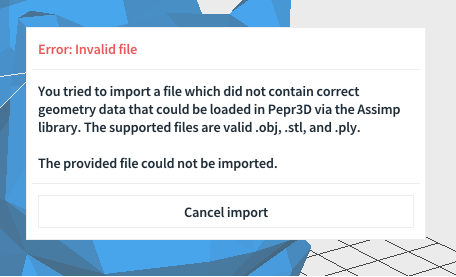
\includegraphics[scale=0.9]{images/invalid_file.png}
	\caption{Loading a file that does not contain any geometry will result in this error.}
	\label{fig:invalidfile}
\end{figure}

\begin{figure}
	\centering
	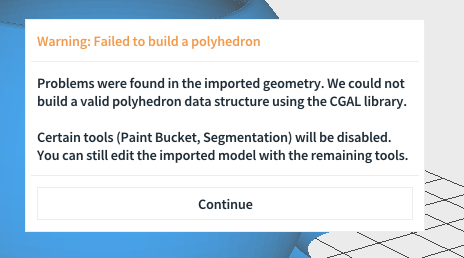
\includegraphics[scale=0.9]{images/polyhedron_failed.png}
	\caption{While this file could be loaded, the file does not conform to a certain assumption of some of the algorithms. Tools using these algorithms will be disabled, but the other tools will work correctly.}
	\label{fig:polyhedronfailed}
\end{figure}

\section{Colouring the model}

Once the model gets loaded, the user is free to select any available tools and color the model as he wishes. We have opted for a quick colouring of triangles, with all four colors. Our result is showcased in Figure \ref{fig:painted}.

\begin{figure}
	\centering
	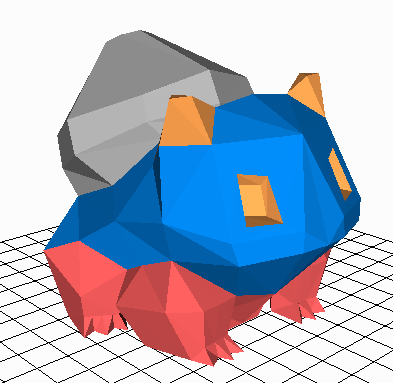
\includegraphics[scale=1]{images/result.png}
	\caption{Our demonstration colouring, achieved by using the Triangle and Bucket painters.}
	\label{fig:painted}
\end{figure}

\section{Exporting the model}

After we are happy with our colouring, we go to the \textbf{Export Assistant}.
This is done by either navigating the menu \textit{File} -- \textit{Export} or clicking the icon from the toolbar.
We are now presented with the user interface seen in Figure \ref{fig:exportui}.
There is a plethora of options here and all the options are described in detail in chapter \ref{ch:impexp}.
For our simple model, we can leave the options to their default values, since $2.5\%$ is a good extrusion throughout the whole print. We also select the checkbox to create a new folder for the exported files.
After that, we select the volumetric export (\textit{depth extrusion}) and select the .STL format for our files.
A new folder is created, containing four different .STL files.
We can now also save the project as the Pepr3D project file -- \textbf{.p3d}, in case we want to alter our colouring later.
We include this coloured model in our attachments.

\begin{figure}
	\centering
	
\includegraphics[scale=0.5]{images/export_ui.png}
	\caption{The demonstration of the GUI of Export Assistant. Here we select the parameters mentioned in the text and can preview all our export options.}
	\label{fig:exportui}
\end{figure}

\section{Putting the files together in Slic3r}

In this section, we showcase how the parts we exported in the previous section look in the Slic3r application. In Figure \ref{fig:slicer}, the model is already loaded into Slic3r. This was done by loading one of the exported .STL files and then adding parts to it, in the \textit{Settings} menu of the object in Slic3r. We can now slice the model, and prove that the Pepr3D export worked correctly.

\begin{figure}
	\centering
	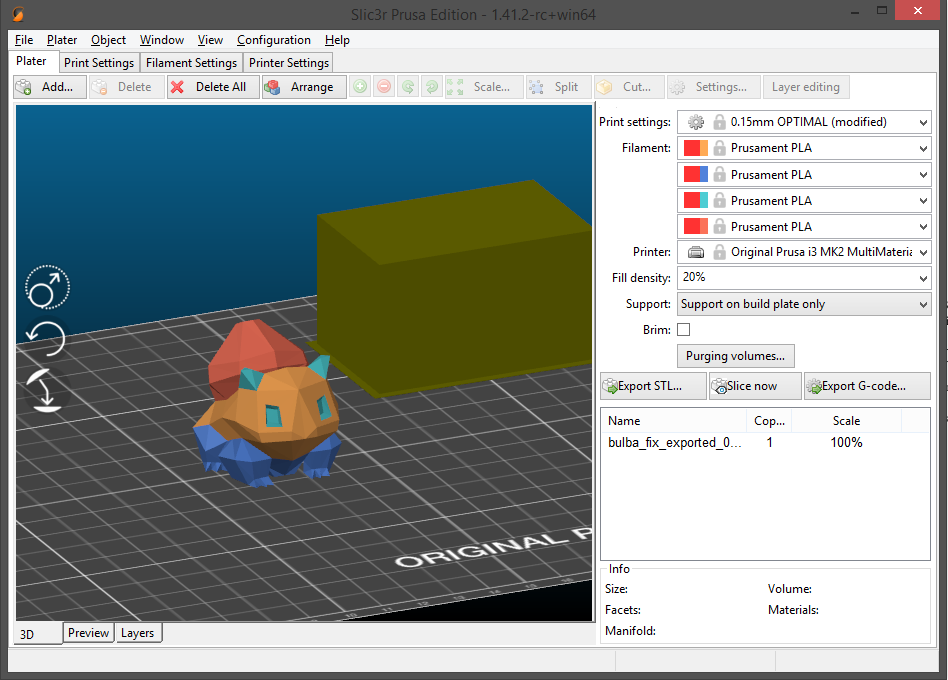
\includegraphics[scale=0.5]{images/slicer.png}
	\caption{The parts exported from Pepr3D loaded correctly into the Slic3r software.}
	\label{fig:slicer}
\end{figure}

\begin{figure}
	\centering
	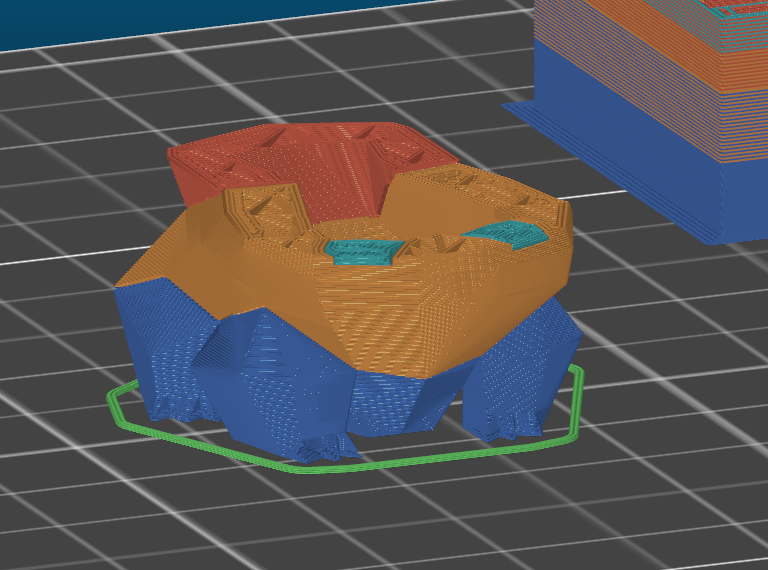
\includegraphics[scale=0.6]{images/sliced.png}
	\caption{The sliced, multimaterial model, ready to be printed.}
	\label{fig:sliced}
\end{figure}

\section{Printing the result}

After we are happy with the slicing we got, as shown in Figure \ref{fig:sliced}, we can print the model. We include a picture finished print of the model in Figure \ref{fig:printed1}, as well as a compilation of other coloured models we printed with our application in Figure \ref{fig:printed2}.

\begin{figure}
	\centering
	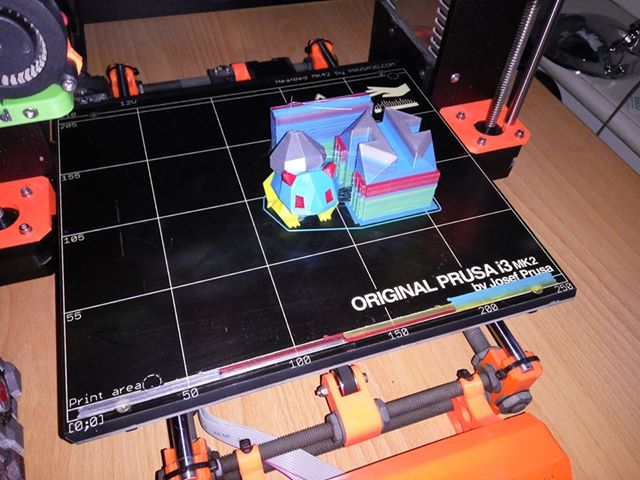
\includegraphics[scale=0.6]{images/printed_bulba.jpg}
	\caption{The printed model, with a custom wipe tower next to it.}
	\label{fig:printed1}
\end{figure}

\vspace{20pt}
\begin{figure}
	\centering
	\centerline{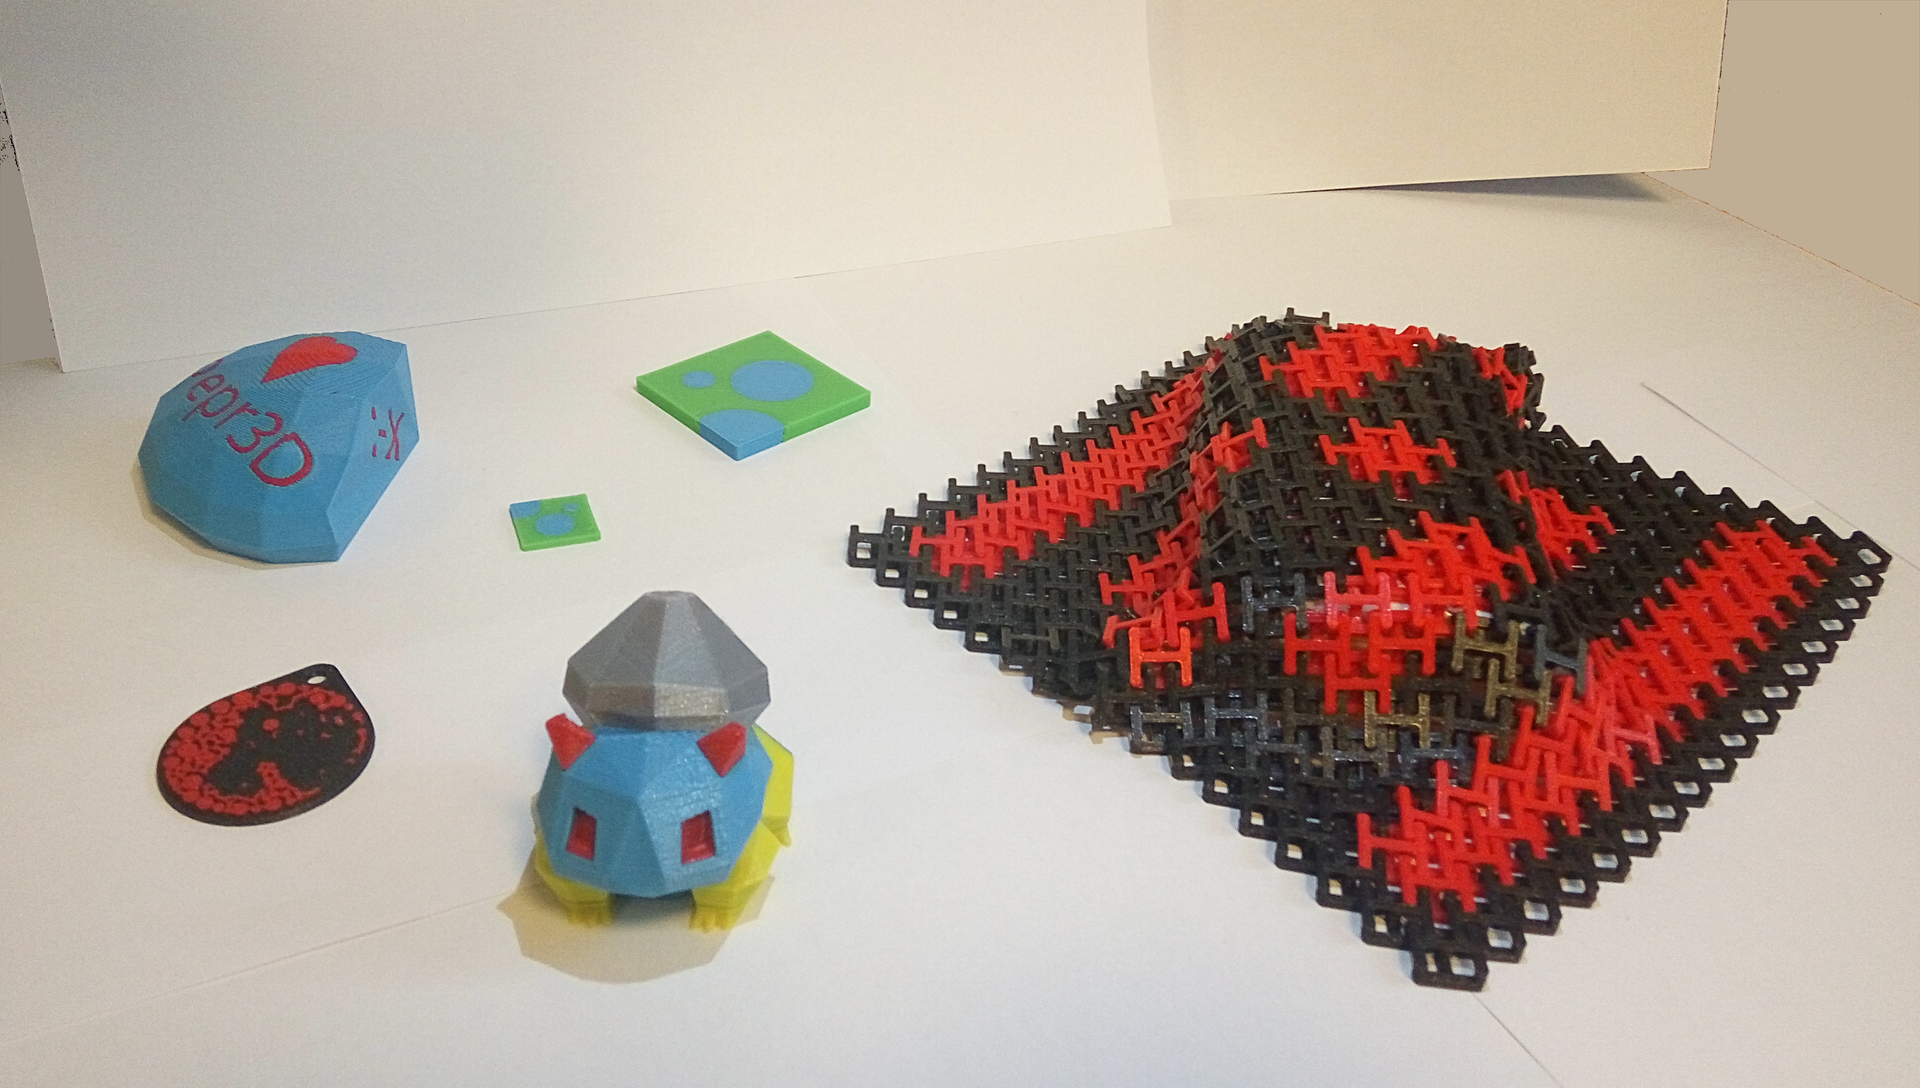
\includegraphics[scale=0.25]{images/results.png}}
	\caption{Other printed models, all painted in Pepr3D.}
	\label{fig:printed2}
\end{figure}

